 \chapter{Testovanie a evaluácia}
\label{kap:tes}

V kapitole Testovanie sa budeme snažiť ukázať schopnosť aplikácie vyhľadávať optimálne cesty s prihliadnutím na meškanie. Správnosť vyhľadaných ciest sa dokazuje ťažko, keďže nemáme k dispozícii porovnateľné dáta. Existujúce aplikácie vyhľadávajú cesty bez prihliadnutia na meškanie. Keďže máme k dispozícii dáta s platnosťou cestovných poriadkov v minulosti a existujúce aplikácie neumožňujú vyhľadávanie v ďalekej minulosti, nevieme porovnať ani vyhľadané cesty bez prihliadnutia na meškanie. 

Vyhľadávací algoritmus sme testovali postupne. Najskôr algoritmus hľadal len jednu najkratšiu cestu nad statickými cestovnými poriadkami. Potom sme algoritmus vylepšili, aby prihliadal aj na meškanie vozidiel. Následne sme upravili vyhľadávanie, aby výsledná cesta nebola len jedna najkratšia, ale viacero optimálnych. Na záver sme upravili algoritmus, aby prihliadal aj na používateľské preferencie zadané pri vyhľadávaní.

Dáta získané od Dopravného podniku Bratislava sú príliš robustné a kontrola algoritmu človekom nad týmito dátami bola nemožná. Vytvorili sme preto testovaciu sadu dát, nad ktorými sme spúšťali vyhľadávanie. Testovacie dáta sme bližšie spomínali v \ref{sec:test-data}. Pre lepší prehľad v testovacích dátach sme nakreslili schému liniek a vygenerovali cestovný poriadok. Algoritmus, ktorý vyhľadával nad testovacími dátami, kontrolovali traja cestujúci. Podľa ich názorov a skúseností sme vytvárali a upravovali filtre. Filtre slúžia na minimalizovanie množiny všetkých ciest, ktoré vedú zo skupiny začiatočných zastávok do konečnej skupiny zastávok. Všetky vyfiltrované cesty však musia byť optimálne.

V nasledujúcich ukážkach znázorníme, ako sa menila množina vyhľadaných ciest v závislosti od vývoja algoritmu.

\subsubsection{Meškanie}
V tejto ukážke môžeme pozorovať, ako sa zmenila vyhľadaná cesta v závislosti od meškania. Na obrázku \ref{fig:test-delay}(a) môžeme vidieť riadok z dát o meškaní vozidiel, ktorý poukazuje na to, že v deň 5.2.2018 v čase 9:59 nadobudla linka $5$ na zastávke Karlova Ves meškanie $1$ minútu. Vyhľadávanie sme spustili 5.2.2018 v čase 10:00. Deň 5.2.2018 je v konfigurácii nastavený ako aktuálny dátum. 

Hľadáme cestu s vyhľadávacími parametrami na obrázku \ref{fig:test-delay}(b). Najskôr algoritmus hľadal len nad statickými cestovnými poriadkami. Našiel preto jednu najrýchlejšiu cestu (obrázok \ref{fig:test-delay}(c)). 
Po tom, ako sme v algoritme začali prihliadať na meškanie vozidiel, zmenil sa aj výsledok vyhľadávania (obrázok \ref{fig:test-delay}(d)). 

Jazda linky $5$ príde na zastávku Botanická záhrada s meškaním a z toho dôvodu sa mení aj prestupná zastávka medzi jazdami. Predvolený minimálny čas na prestup medzi linkami je $1$ minúta. Keďže jazda linky $5$ má meškanie, cestujúci by nemal žiadny čas na prestup na zastávke Vysoká, Tchibo Outlet. Prestupnou zastávkou sa preto stala zastávka Poštová - Martinus.

Všimnime si ešte označenie meškania. Meškajúca jazda má zafarbené časy červenou farbou. Po kliknutí na detail (obrázok \ref{fig:test-delay}(e)) vidíme aj hodnotu meškania jazdy. Časy z druhej jazdy sú čiernou farbou, pretože táto jazda ešte nevyrazila zo začiatočnej zastávky v čase vyhľadávania. 

\begin{figure}[H]
\centerline{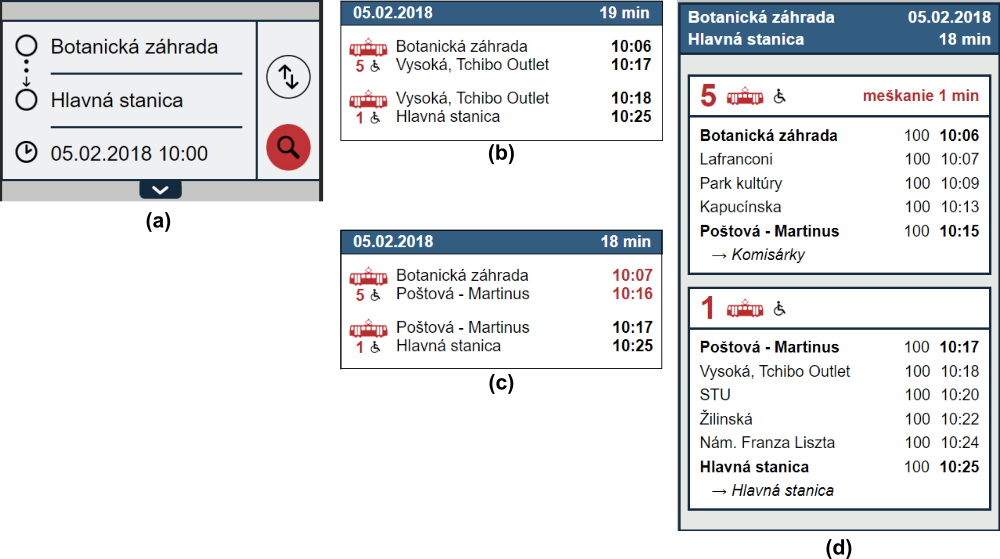
\includegraphics[width=1.0\textwidth]{images/test/delay}}
\caption[Testovanie meškania]{Testovanie meškania}
\label{fig:test-delay}
\end{figure}

\subsubsection{Alternatívne cesty}
Následne sme vylepšili vyhľadávanie tak, aby aplikácia cestujúcemu ponúkla vždy alternatívne optimálne cesty. Prihliadame už aj na meškanie spojov. Spustili sme vyhľadávanie s parametrami na obrázku \ref{fig:test-alternative}(a). Doteraz aplikácia vracala iba jednu najrýchlejšiu cestu a so zadanými parametrami by bola vyhľadaná cesta na obrázku \ref{fig:test-alternative}(b).

Po vylepšení vyhľadávania nám aplikácia ponúkla množinu ciest, ktoré sú na obrázku \ref{fig:test-alternative}(c). Vidíme prvú najrýchlejšiu cestu s $2$ prestupmi, druhú pomalšiu s jedným prestupom a tretiu s najhorším časom príchodu do cieľa bez nutnosti prestupu. 

Vo filtrovacom mechanizme ciest je podmienka, že najrýchlejšiu cestu zobrazujeme vždy. Cesty z neskoršími príchodmi do cieľa zobrazujeme len vtedy, ak majú menej prestupov. Avšak nemôžu prísť do cieľa s veľkým oneskorením po najrýchlejšej ceste. Rozdiel v časoch musí byť menší alebo rovný, ako rozdiel počtu prestupov vynásobený $m$ minútami. V projekte sme si určili $m = 5$ minút. Najrýchlejšou cestou je prvá cesta na obrázku \ref{fig:test-alternative}(c). Rozdiel v prestupoch prvej a druhej cesty je $1$ a rozdiel v časoch príchodu do cieľa sú $3$ minúty ($3$ minúty $\leq 1\times5$ minút).
Rozdiel v prestupoch medzi prvou a treťou cestou sú $2$ prestupy a rozdiel v časoch príchodu do cieľa je $8$ ($8$ minút $\leq 2\times5$ minút).

Na obrázkoch \ref{fig:test-alternative}(b) a (c) si môžeme všimnúť zafarbené časy zelenou farbou. Čo znamená, že jazda linky už vyrazila z prvej zastávky a nemá žiadne meškanie. V detaile prvej cesty (obrázok \ref{fig:test-alternative}(d)) môžeme vidieť označenie "včas" pri nemeškajúcej jazde.

\begin{figure}[H]
\centerline{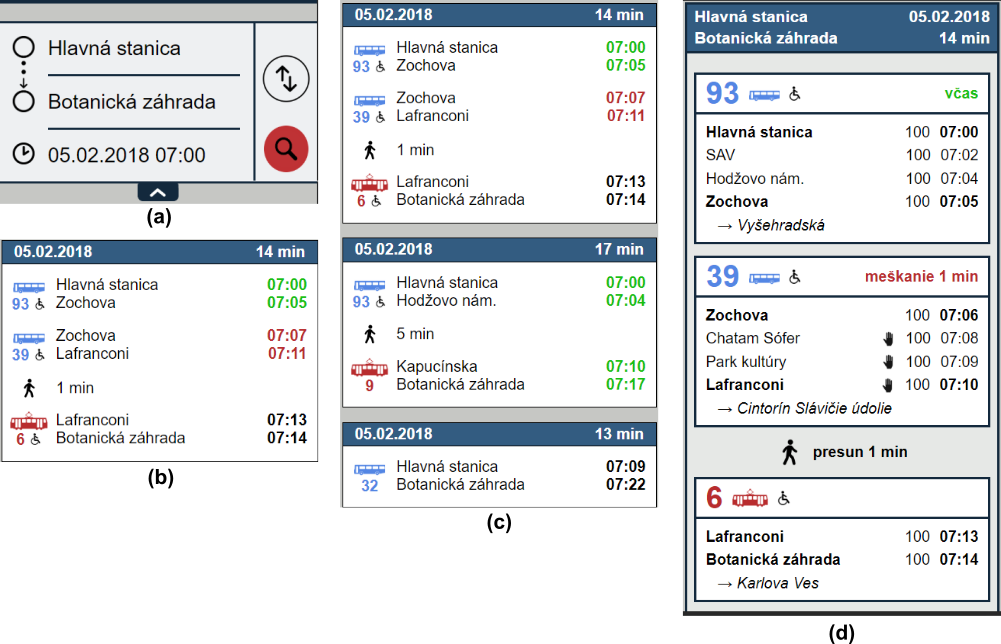
\includegraphics[width=1.0\textwidth]{images/test/alternative}}
\caption[Testovanie alternatívnych ciest]{Testovanie alternatívnych ciest}
\label{fig:test-alternative}
\end{figure}

\subsubsection{Meškanie a alternatívne cesty}
Pomocou nasledujúcej ukážky znázorníme, aký vplyv má meškanie na zobrazenie optimálnych ciest. Na obrázku \ref{fig:test-delay-alternative}(a) vidíme vyhľadávacie parametre. Najskôr sme definovali v systéme aktuálny deň 4.2.2018, aby získané meškania pri vyhľadávaní 5.2.2018 nemali vplyv na vyhľadávanie. Aplikácia ponúkla jednu vyhovujúci cestu a žiadne alternatívne optimálne cesty (obrázok \ref{fig:test-delay-alternative} (a)). 

Potom sme zmenili dátum v systéme na 5.2.2018 a čas 6:00. Teraz už algoritmus prihliada na meškania, ktoré vznikli do 6:00 hodiny. Jazda linky $5$ má minútové meškanie (označené červenou farbou). Zaujímavé však je, že pribudla aj alternatívna cesta, ktorá nevyžaduje začiatočný peší presun. V predchádzajúcom hľadaní bola táto cesta odfiltrovaná. Potrebný peší presun na začiatku tiež penalizujeme ako prestup. 
 
V prípade \ref{fig:test-delay-alternative}(b) bola priama cesta odfiltrovaná, pretože rozdiel v časoch príchodu do cieľa je väčší ako rozdiel v počte prestupov vynásobaných 5 minútami ($6$ minút $\leq 1\times5$ minút).
V prípade \ref{fig:test-delay-alternative}(c) je už rozdiel v časoch rovných $5$ minút. Preto cesta s menším počtom prestupov nebola vyfiltrovaná.

\begin{figure}[H]
\centerline{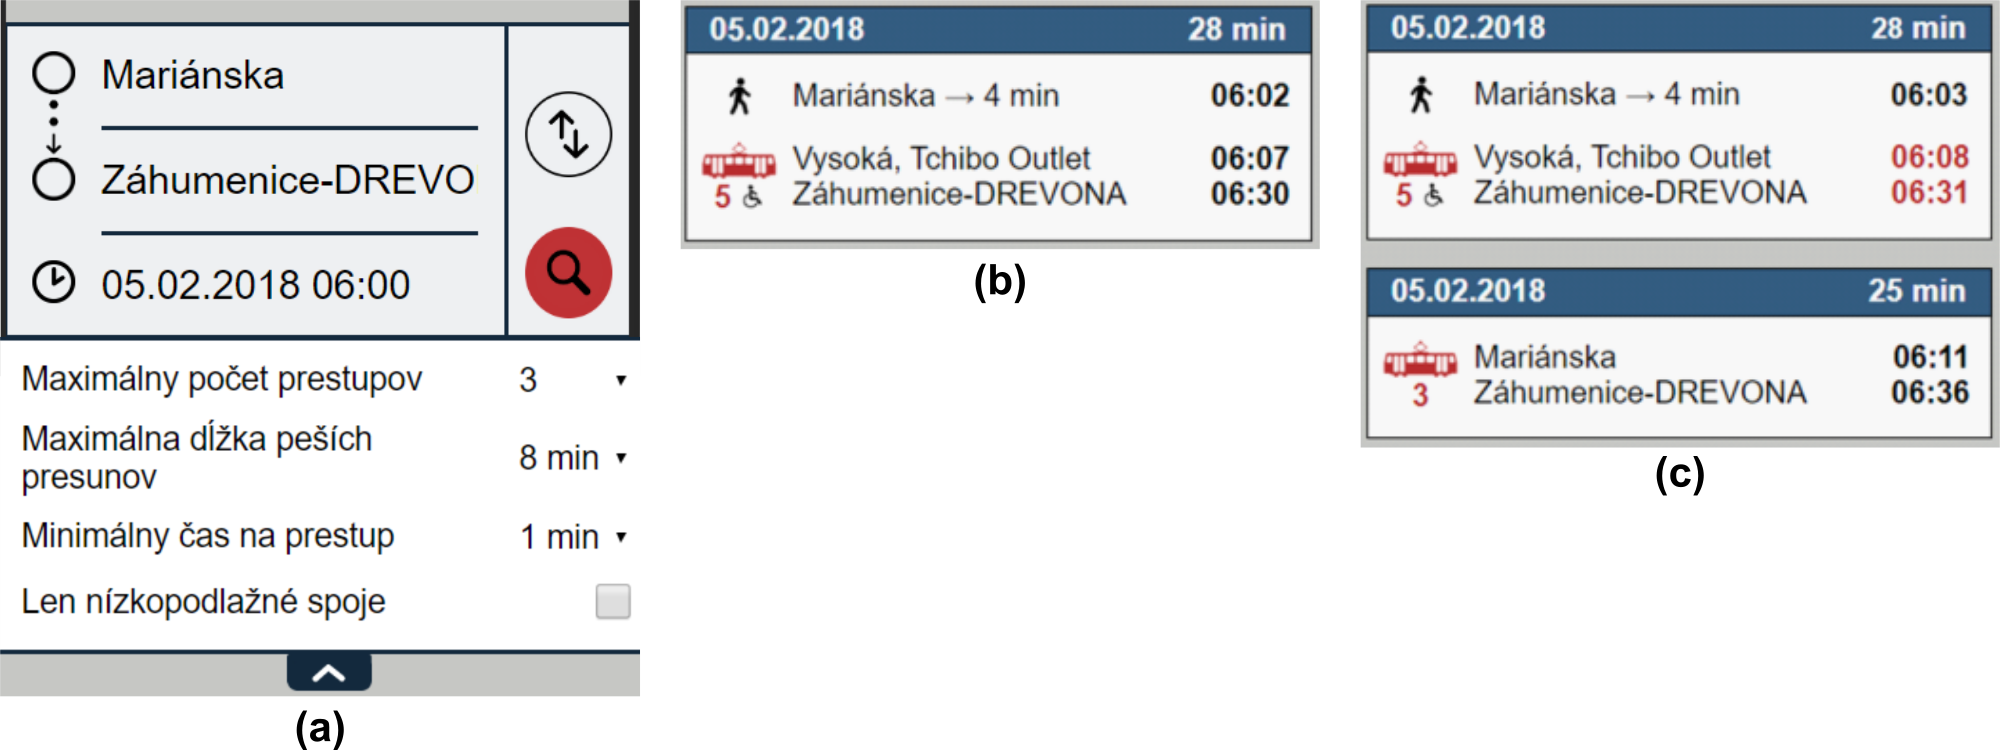
\includegraphics[width=1.0\textwidth]{images/test/delay-alternative}}
\caption[Testovanie meškania a alternatívnych ciest]{Testovanie meškania a alternatívnych ciest}
\label{fig:test-delay-alternative}
\end{figure}

\subsubsection{Používateľské preferencie}

V aplikácii môže používateľ nastaviť okrem základných vyhľadávaích parametrov aj ďalšie parametre. Nachádzajú sa vo vysúvacej lište pod povinnými vyhľadávacími parametrami. Ďalej sme upravili algoritmus, aby počas vyhľadávania ciest prihliadal na zadané prídavné parametre. Na obrázku \ref{fig:test-max-transfers}(a) môžeme vidieť zadané parametre vyhľadávania. Všimnime si najmä, že maximálny počet prednastavený na hodnotu $3$ a začiatočný bod nie je zastávka, ale aktuálna poloha používateľa. 

Vyhľadané cesty (obrázok \ref{fig:test-max-transfers}(b)) sú dve. Jedna cesta obsahuje $1$ prestup a druhá neobsahuje žiadny. Po zmene vyhľadávacích parametrov (obrázok \ref{fig:test-max-transfers}(c)) je vyhľadaná cesta už len jedna – tá bez prestupu (obrázok \ref{fig:test-max-transfers}(d)).

\begin{figure}[H]
\centerline{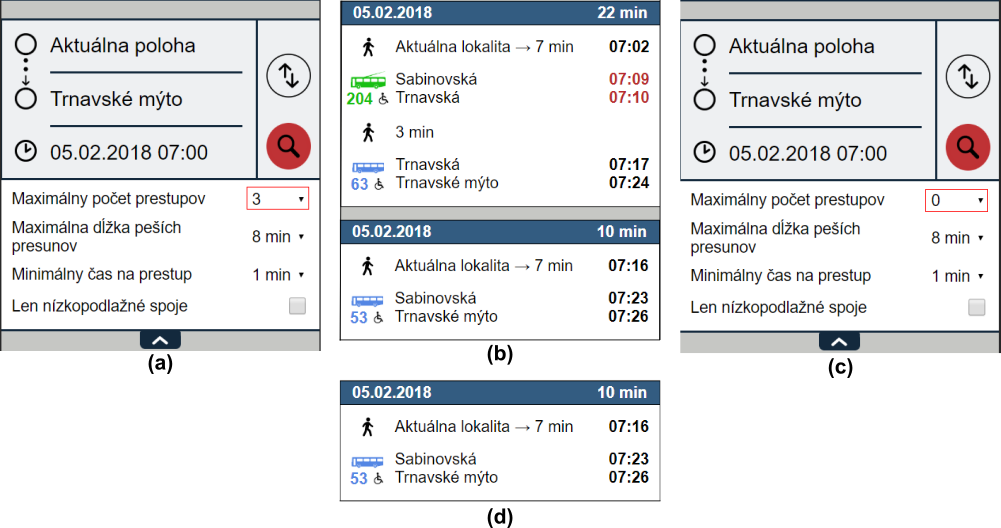
\includegraphics[width=1.0\textwidth]{images/test/max-transfers-act}}
\caption[Testovanie obmedzenia počtu prestupov]{Testovanie obmedzenia počtu prestupov}
\label{fig:test-max-transfers}
\end{figure}

Na ďalšom obrázku ukážeme, ako sa algoritmus vysporiadava s obmedzením dĺžky pešieho presunu. Po zadaní parametrov na obrázku \ref{fig:test-max-walking}(a) aplikácia ponúkla cesty na obrázku \ref{fig:test-max-walking}(b). Tu vidíme ponuku dvoch optimálnych ciest. Prvá cesta je najrýchlejšia, ale obsahuje dva pešie presuny. Druhá cesta obsahuje len jeden peší presun. 
Následne sme zmenili vo vyhľadávacích parametroch hodnotu maximálnej dĺžky pešieho presunu na $4$ minúty (obrázok \ref{fig:test-max-walking}(c)). Na obrázku \ref{fig:test-max-walking}(d) môžeme vidieť vyhľadanú jednu cestu. Najrýchlejšia cesta bola vyfiltrovaná, keďže obsahovala $6$ – minútový peší presun. 

\begin{figure}[H]
\centerline{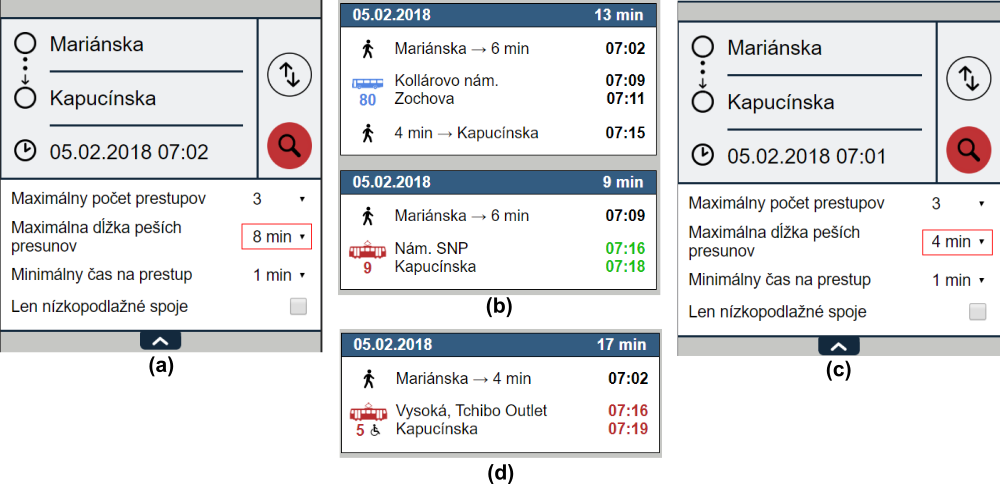
\includegraphics[width=1.0\textwidth]{images/test/max-walking}}
\caption[Testovanie obmedzenia dĺžky peších presunov]{Testovanie obmedzenia dĺžky peších presunov}
\label{fig:test-max-walking}
\end{figure}

V ďalšej ukážke znázorníme fungovanie nastavenia minimálneho času na prestup. 
\\ \\
Na obrázku \ref{fig:test-min-transfer}(a) je hodnota minimálneho času na prestup nastavená na hodnotu $1$. Vyhľadaná cesta (obrázok \ref{fig:test-min-transfer}(b)) vyžaduje $1$ prestup a čas na prestup medzi linkami je $1$ minúta. Po tom, ako sme zmenili hodnotu minimálneho času na prestup na hodnotu $3$ vo vyhľadávacích parametroch (obrázok \ref{fig:test-min-transfer}(c)), dostávame inú vyhľadanú cestu s jedným prestupom (obrázok \ref{fig:test-min-transfer}(d)). Na prestup medzi zastávkami má cestujúci $4$ minúty.

\begin{figure}[H]
\centerline{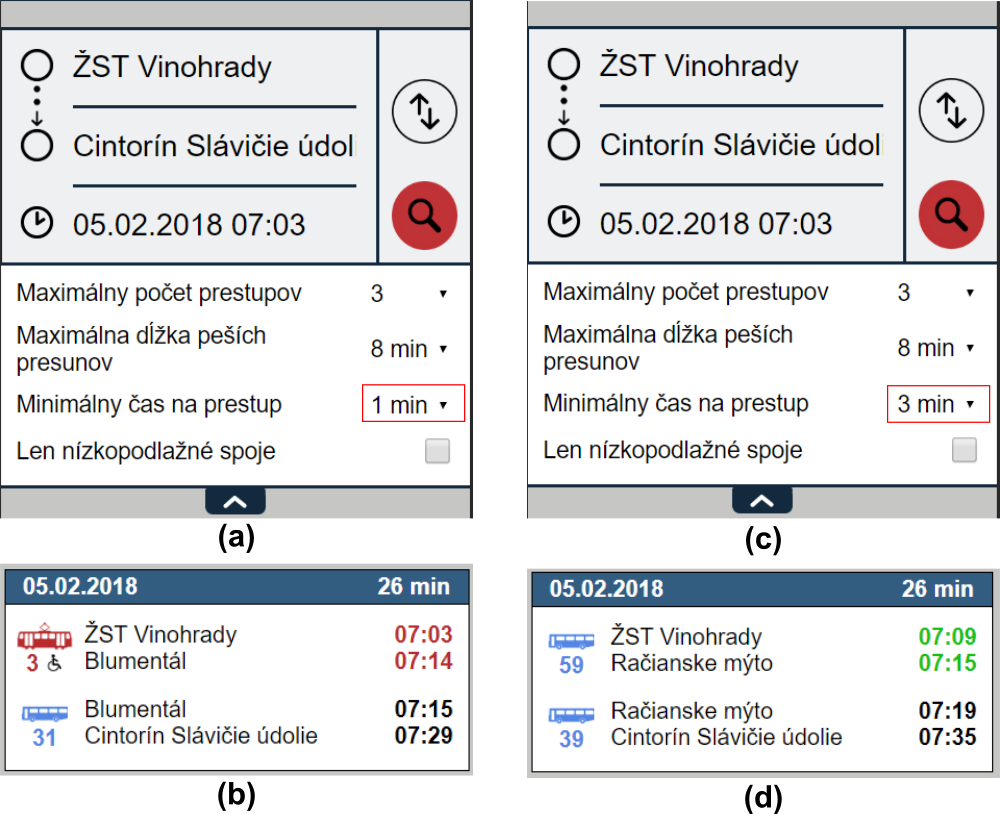
\includegraphics[width=0.7\textwidth]{images/test/min-transfer}}
\caption[Testovanie minimálneho času na prestup]{Testovanie minimálneho času na prestup}
\label{fig:test-min-transfer}
\end{figure}

V poslednej ukážke dokážeme fungovanie vyhľadávania s prihliadnutím na obmedzenie len nízkopodlažných vozidiel. Na obrázku \ref{fig:test-low-floor}(a) vidíme zobrazené parametre vyhľadávania a na obrázku (b) vidíme vyhľadanú cestu. Cesta obsahuje $2$ prestupy a je zložená z troch jázd. Len pre jednu z jázd tejto cesty platí, že má priradené nízkopodlažné vozidlo. Po zmene vyhľadávacích parametrov (obrázok \ref{fig:test-low-floor}(c)) je vyhľadaná iná cesta (obrázok \ref{fig:test-low-floor}(d)). Táto cesta obsahuje $2$ jazdy, pričom obe jazdy majú priradené nízkopodlažné vozdilo.

\begin{figure}[H]
\centerline{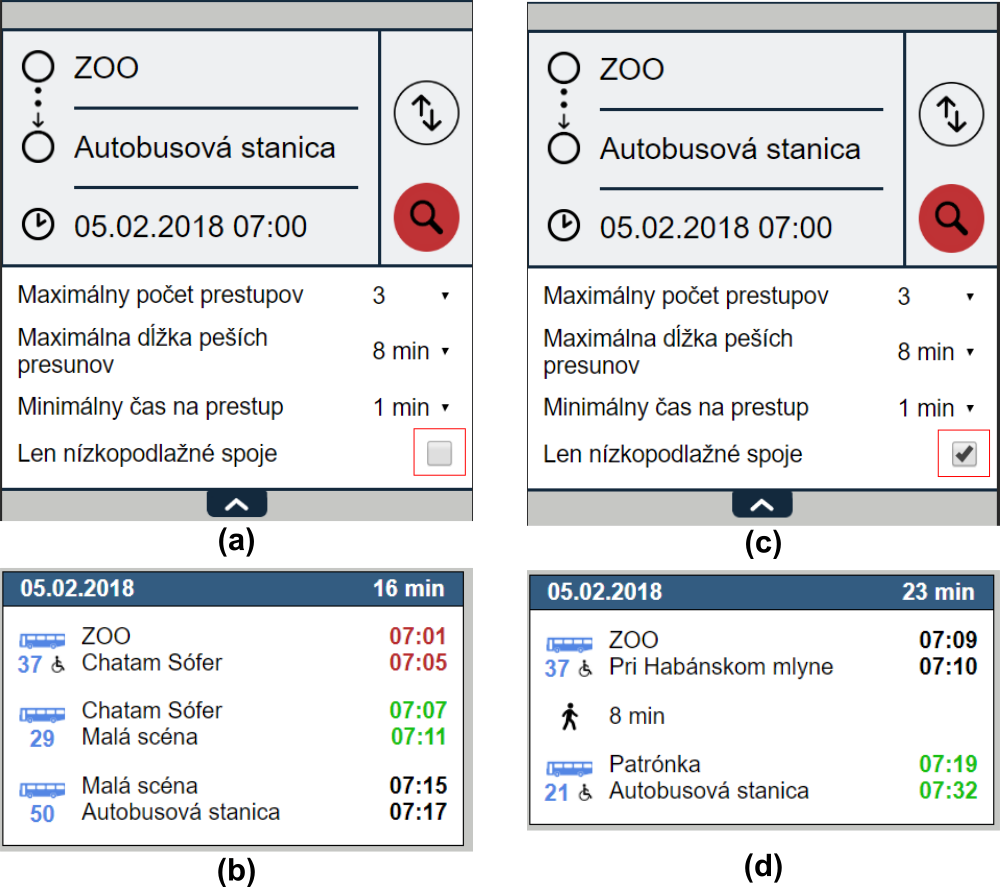
\includegraphics[width=0.7\textwidth]{images/test/low-floor}}
\caption[Testovanie hľadania len nízkopodlažných vozidiel]{Testovanie hľadania len nízkopodlažných vozidiel}
\label{fig:test-low-floor}
\end{figure}





